% Measurement results / analysis / discussion:
% whatever you have done, you must comment it, compare it to other systems, evaluate it
% usually, adequate graphs help to show the benefits of your approach
% caution: each result/graph must be discussed! what’s the reason for this peak or why have you ovserved this effect


% Experiments
% Data
    % 33 days
    % 138 - pair in BTC market
    % 47 Gb
    % 5 sec.
    % ccxt, binance, coinmarketcap
    
% step 1
    % Use anomaly detection algorithm
    % Filter anomalies
    
% step 2
    % clean data
    % remove inconsistent data

% step 3
    % feature engineering (create new features)
    % normalize

% step 4
    % Dim reduction
    
% step 5
    % train - evaluate
    
\chapter{Evaluation}\label{ch:evaluation}\glsresetall
TBW
\section{Experimental Setup}

\section{Results}
\begin{table}[H]
        \centering
        \begin{tabularx}{\textwidth}{ |R|R||R|R||R|R| }
                \multicolumn{2}{c}{WABI-BTC} & \multicolumn{2}{c}{MITH-BTC} & \multicolumn{2}{c}{ETH-BTC} \\\hline
                $\numprint{376}$\cellcolor{green!91} & $\numprint{36}$\cellcolor{red!9} & $\numprint{0}$\cellcolor{green!0} & $\numprint{2}$\cellcolor{red!100} & $\numprint{0}$\cellcolor{green!100} & $\numprint{0}$\cellcolor{red!0} \\
                $\numprint{23440}$\cellcolor{red!5} & $\numprint{531622}$\cellcolor{green!95} & $\numprint{26798}$\cellcolor{red!5} & $\numprint{528675}$\cellcolor{green!95} & $\numprint{0}$\cellcolor{red!0} & $\numprint{555474}$\cellcolor{green!100} \\
                \hline
                \addlinespace[.2cm]

                \multicolumn{2}{c}{XRP-BTC} & \multicolumn{2}{c}{BTT-BTC} & \multicolumn{2}{c}{OST-BTC} \\\hline               
                $\numprint{0}$\cellcolor{green!100} & $\numprint{0}$\cellcolor{red!0} & $\numprint{0}$\cellcolor{green!100} & $\numprint{0}$\cellcolor{red!0} & $\numprint{488}$\cellcolor{green!90} & $\numprint{53}$\cellcolor{red!10} \\
                $\numprint{0}$\cellcolor{red!0} & $\numprint{555474}$\cellcolor{green!100} & $\numprint{3400}$\cellcolor{red!1} & $\numprint{552074}$\cellcolor{green!99} & $\numprint{8705}$\cellcolor{red!2} & $\numprint{546228}$\cellcolor{green!98} \\
                \hline
                \addlinespace[.2cm]

                \multicolumn{2}{c}{CDT-BTC} & \multicolumn{2}{c}{GNT-BTC} & \multicolumn{2}{c}{TRX-BTC} \\\hline               
                $\numprint{407}$\cellcolor{green!88} & $\numprint{51}$\cellcolor{red!12} & $\numprint{375}$\cellcolor{green!78} & $\numprint{105}$\cellcolor{red!22} & $\numprint{0}$\cellcolor{green!100} & $\numprint{0}$\cellcolor{red!0} \\
                $\numprint{18303}$\cellcolor{red!4} & $\numprint{536713}$\cellcolor{green!96} & $\numprint{20994}$\cellcolor{red!4} & $\numprint{534000}$\cellcolor{green!96} & $\numprint{289}$\cellcolor{red!1} & $\numprint{555185}$\cellcolor{green!99} \\
                \hline
                \addlinespace[.2cm]

                \multicolumn{2}{c}{MTH-BTC} & \multicolumn{2}{c}{DLT-BTC} & \multicolumn{2}{c}{SC-BTC} \\\hline                
                $\numprint{487}$\cellcolor{green!97} & $\numprint{16}$\cellcolor{red!3} & $\numprint{584}$\cellcolor{green!87} & $\numprint{85}$\cellcolor{red!13} & $\numprint{0}$\cellcolor{green!100} & $\numprint{0}$\cellcolor{red!0} \\
                $\numprint{12032}$\cellcolor{red!3} & $\numprint{542939}$\cellcolor{green!97} & $\numprint{19223}$\cellcolor{red!3} & $\numprint{535580}$\cellcolor{green!97} & $\numprint{7234}$\cellcolor{red!2} & $\numprint{548240}$\cellcolor{green!98} \\
                \hline
                \addlinespace[.2cm]

                \multicolumn{2}{c}{SNT-BTC} & \multicolumn{2}{c}{XEM-BTC} & \multicolumn{2}{c}{VIB-BTC} \\\hline                
                $\numprint{323}$\cellcolor{green!88} & $\numprint{40}$\cellcolor{red!12} & $\numprint{0}$\cellcolor{green!100} & $\numprint{0}$\cellcolor{red!0} & $\numprint{674}$\cellcolor{green!99} & $\numprint{7}$\cellcolor{red!1} \\
                $\numprint{8138}$\cellcolor{red!2} & $\numprint{546973}$\cellcolor{green!99} & $\numprint{914}$\cellcolor{red!1} & $\numprint{554559}$\cellcolor{green!99} & $\numprint{22358}$\cellcolor{red!5} & $\numprint{532435}$\cellcolor{green!95} \\
                \hline
                \addlinespace[.2cm]

                \multicolumn{2}{c}{MTL-BTC} & \multicolumn{2}{c}{HC-BTC} & \multicolumn{2}{c}{STORM-BTC} \\\hline             
                $\numprint{477}$\cellcolor{green!93} & $\numprint{36}$\cellcolor{red!7} & $\numprint{251}$\cellcolor{green!57} & $\numprint{188}$\cellcolor{red!43} & $\numprint{0}$\cellcolor{green!100} & $\numprint{0}$\cellcolor{red!0} \\
                $\numprint{29687}$\cellcolor{red!6} & $\numprint{525274}$\cellcolor{green!94} & $\numprint{5213}$\cellcolor{red!1} & $\numprint{549822}$\cellcolor{green!99} & $\numprint{14995}$\cellcolor{red!3} & $\numprint{540479}$\cellcolor{green!97} \\
                \hline
                \addlinespace[.2cm]

                \multicolumn{2}{c}{INS-BTC} & \multicolumn{2}{c}{LUN-BTC} & \multicolumn{2}{c}{NXS-BTC} \\\hline               
                $\numprint{0}$\cellcolor{green!0} & $\numprint{1}$\cellcolor{red!100} & $\numprint{792}$\cellcolor{green!93} & $\numprint{57}$\cellcolor{red!7} & $\numprint{0}$\cellcolor{green!100} & $\numprint{0}$\cellcolor{red!0} \\
                $\numprint{7032}$\cellcolor{red!2} & $\numprint{548439}$\cellcolor{green!98} & $\numprint{12443}$\cellcolor{red!3} & $\numprint{542182}$\cellcolor{green!97} & $\numprint{6554}$\cellcolor{red!1} & $\numprint{548920}$\cellcolor{green!99} \\
                \hline
                \addlinespace[.2cm]

                \multicolumn{2}{c}{TNB-BTC} & \multicolumn{2}{c}{NPXS-BTC} & \multicolumn{2}{c}{ZRX-BTC} \\\hline               
                $\numprint{441}$\cellcolor{green!99} & $\numprint{3}$\cellcolor{red!1} & $\numprint{0}$\cellcolor{green!100} & $\numprint{0}$\cellcolor{red!0} & $\numprint{0}$\cellcolor{green!100} & $\numprint{0}$\cellcolor{red!0} \\
                $\numprint{47144}$\cellcolor{red!9} & $\numprint{507886}$\cellcolor{green!91} & $\numprint{3381}$\cellcolor{red!1} & $\numprint{552093}$\cellcolor{green!99} & $\numprint{10138}$\cellcolor{red!2} & $\numprint{545336}$\cellcolor{green!98} \\
                \hline
                \addlinespace[.2cm]

                \multicolumn{2}{c}{VET-BTC} & \multicolumn{2}{c}{RCN-BTC} & \multicolumn{2}{c}{ETC-BTC} \\\hline                
                $\numprint{0}$\cellcolor{green!100} & $\numprint{0}$\cellcolor{red!0} & $\numprint{487}$\cellcolor{green!95} & $\numprint{26}$\cellcolor{red!5} & $\numprint{160}$\cellcolor{green!84} & $\numprint{30}$\cellcolor{red!16} \\
                $\numprint{1321}$\cellcolor{red!2} & $\numprint{554153}$\cellcolor{green!98} & $\numprint{10697}$\cellcolor{red!2} & $\numprint{544264}$\cellcolor{green!98} & $\numprint{2890}$\cellcolor{red!1} & $\numprint{552394}$\cellcolor{green!99} \\
                \hline
                \addlinespace[.2cm]

                \multicolumn{2}{c}{SNM-BTC} & \multicolumn{2}{c}{SKY-BTC} & \multicolumn{2}{c}{LOOM-BTC} \\\hline              
                $\numprint{1209}$\cellcolor{green!95} & $\numprint{55}$\cellcolor{red!5} & $\numprint{141}$\cellcolor{green!76} & $\numprint{44}$\cellcolor{red!24} & $\numprint{0}$\cellcolor{green!100} & $\numprint{0}$\cellcolor{red!0} \\
                $\numprint{21950}$\cellcolor{red!4} & $\numprint{532260}$\cellcolor{green!96} & $\numprint{14423}$\cellcolor{red!2} & $\numprint{540866}$\cellcolor{green!98} & $\numprint{1485}$\cellcolor{red!1} & $\numprint{553989}$\cellcolor{green!99} \\
                \hline
                \addlinespace[.2cm]

                \multicolumn{2}{c}{CVC-BTC} & \multicolumn{2}{c}{PHX-BTC} & \multicolumn{2}{c}{PPT-BTC} \\\hline               
                $\numprint{238}$\cellcolor{green!76} & $\numprint{74}$\cellcolor{red!24} & $\numprint{0}$\cellcolor{green!0} & $\numprint{1}$\cellcolor{red!100} & $\numprint{0}$\cellcolor{green!0} & $\numprint{1}$\cellcolor{red!100} \\
                $\numprint{8393}$\cellcolor{red!1} & $\numprint{546769}$\cellcolor{green!99} & $\numprint{13211}$\cellcolor{red!2} & $\numprint{542262}$\cellcolor{green!98} & $\numprint{6010}$\cellcolor{red!1} & $\numprint{549463}$\cellcolor{green!99} \\
                \hline
        \end{tabularx}
        \caption[\project's confusion matrices of tested markets]{confusion matrices of the $33$ tested markets.}
        \label{tab:results}
\end{table}
\begin{table}
    \centering
    \begin{tabular}{|c|c|c|c|}\hline
                &   \multicolumn{3}{c|}{Predicted class}\\\hline
    True class  &  Positive             & Negative              & Total \\\hline
    Positive    & $tp$: true positive   & $fn$: false negative  & $p$   \\
    Negative    & $fp$: false positive  & $tn$: true negative   & $n$   \\\hline
    Total       & $p'$                  & $n'$                  & $N$   \\\hline
    \end{tabular}
    \caption{Confusion matrix}
    \label{tab:confmat}
\end{table}
\begin{table}
        \centering
        \begin{tabularx}{\textwidth}{ |R|R|R|R| }\hline
                    &   \multicolumn{3}{c|}{Predicted class}\\\hline
        True class  & Positive              & Negative              & Total                 \\\hline
        Positive    & $\numprint{7910}$     & $\numprint{911}$      & $\numprint{8821}$     \\
        Negative    & $\numprint{388795}$   & $\numprint{17933021}$ & $\numprint{18321816}$ \\\hline
        Total       & $\numprint{396705}$   & $\numprint{17933932}$ & $\numprint{18330637}$ \\\hline
        \end{tabularx}
        \caption{\project's confusion matrix}
        \label{tab:model_performance}
\end{table}
\begin{table}
    \centering
    \begin{tabular}{|c|c|r|}\hline
    Name        & Formula       &   Result      \\\hline
    error       & $(fp+fn)/N$   &   $0.0217$    \\
    accuracy    & $(tp+tn)/N$   &   $0.9782$    \\\hline
    tp-rate     & $tp/p$        &   $0.8967$    \\
    fp-rate     & $fp/n$        &   $0.0212$    \\\hline
    sensitivity & $tp/p$        &   $0.8967$    \\
    specificity & $tn/n$        &   $0.9787$    \\\hline
    recall      & $tp/p$        &   $0.8967$    \\
    precision   & $tp/p'$       &   $0.0199$    \\\hline
    \end{tabular}
    \caption{Performance measure}
    \label{tab:performance}
\end{table}
\begin{figure}
    \centering
    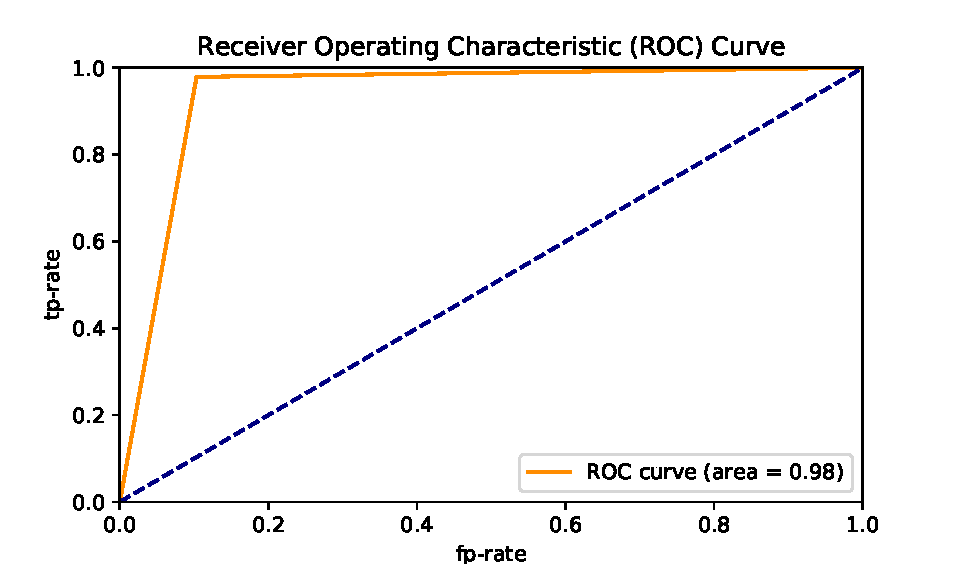
\includegraphics[width=\textwidth]{results/roc.pdf}
    \caption{Roc Curve}
    \label{fig:my_label}
\end{figure}
\begin{align}\label{eq:f_score}
    F_\beta &= (1+\beta^2) \cdot \frac{\text{precision} \cdot \text{recall}}{(\beta^2\cdot\text{precision}) + \text{recall}},\quad
    \begin{cases} 
    F_{0.5} &= 0.0247\\ 
    F_1     &= 0.0389\\ 
    F_2     &= 0.0912\\ 
    \end{cases}
\end{align}